% What drew what: a macro, a loop, a multi-line statement and plots, each tied to its code.
\documentclass{standalone}
\usepackage{tikz,pgfplots}
\newcommand{\card}[2]{\node[draw, fill=blue!10] at (#1,0) {#2};}
\begin{document}
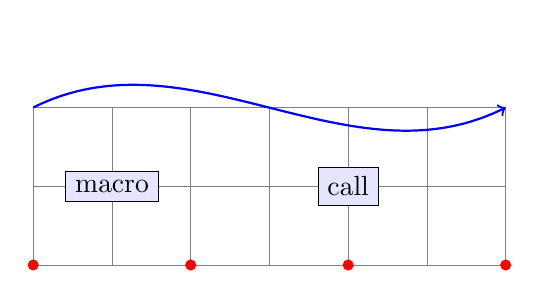
\begin{tikzpicture}
  \draw[help lines] (0,-1) grid (6,1);
  \card{1}{macro}
  \card{4}{call}
  \foreach \x in {0,2,4,6} {
    \fill[red] (\x,-1) circle (2pt);
  }
  \draw[->, thick, blue]
    (0,1) .. controls (2,2) and (4,0) ..
    (6,1);
\end{tikzpicture}
\quad
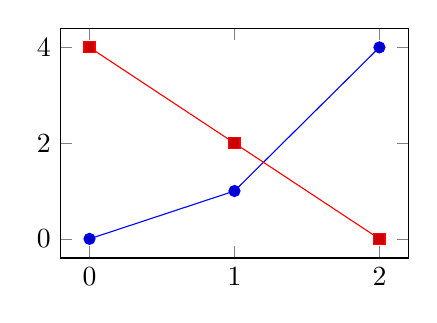
\begin{tikzpicture}
  \begin{axis}[width=6cm, height=4.5cm]
    \addplot coordinates {(0,0) (1,1) (2,4)};
    \addplot coordinates {(0,4) (1,2) (2,0)};
  \end{axis}
\end{tikzpicture}
\end{document}
